\documentclass[11pt]{article}

% ── Packages ────────────────────────────────────────────────
\usepackage[margin=1in]{geometry}
\usepackage{amsmath, amssymb, amsthm}
\usepackage{booktabs}
\usepackage{graphicx}
\usepackage{hyperref}
\usepackage{natbib}
\usepackage{setspace}
\usepackage{microtype}
\usepackage{enumitem}
\usepackage{caption}
\usepackage{subcaption}
\usepackage{xcolor}
\usepackage{float}
% code packages
\usepackage{listings}
\usepackage{inconsolata}
\lstset{basicstyle=\ttfamily\footnotesize,breaklines=true}
\usepackage{csvsimple}
\usepackage{booktabs}

% ── Hyperref setup ──────────────────────────────────────────
\hypersetup{
    colorlinks = true,
    linkcolor  = black,
    citecolor  = black,
    urlcolor   = blue
}

% ── Theorem environments ────────────────────────────────────
\newtheorem{theorem}{Theorem}
\newtheorem{proposition}{Proposition}
\newtheorem{lemma}{Lemma}
\newtheorem{corollary}{Corollary}
\theoremstyle{definition}
\newtheorem{definition}{Definition}
\newtheorem{assumption}{Assumption}
\theoremstyle{remark}
\newtheorem{remark}{Remark}

% ── Spacing ─────────────────────────────────────────────────
\onehalfspacing

% ── Title block ─────────────────────────────────────────────
\title{Love of Variety: Switching Stats}
\author{Tate Mason}
\date{\today}

% ============================================================
\begin{document}
\maketitle
\thispagestyle{empty}

\section{Overview}

My main update is around switching behavior of consumers. I have been mostly
concerned with two things: length of switch and type of switch. To spoil, households will,
on average, switch for about 1-1.5 periods. Further, most of the switching is
from plain yogurt to some other flavor. I have left it as 12 flavors, as I worry
I will be too zoomed out going to the proposed "berry, plain, other" setup, but
if this is a major point, it would not be a problem to implement. Below, I will
provide stats and a couple of graphs, as well as some definitions so the graphs
are more interpretable. 

\section{Definitions and Statistics}

Flavors are as follows:

\begin{centering}
  \begin{enumerate}
    \item Apple
    \item Blueberry
    \item Banana
    \item Cherry
    \item Key Lime
    \item Lemon
    \item Peach
    \item Raspberry
    \item Strawberry
    \item Vanilla
    \item Mixed Flavors
    \item Plain
  \end{enumerate}
\end{centering}

Statistics given before, updated from coding changes:

\begin{table}[htbp]
    \centering
    \caption{Descriptive Statistics}
    \label{tab:desc_stats}
    \begin{tabular}{lc}
        \toprule
        Statistic & Value \\
        \midrule
        \# Households               & 7169 \\
        Mean \# Times Observed      & 8.77 \\
        Yogurt Purchases            & 1.98 \\
        Mean Income                 & \$17,164 \\
        Median Income               & \$17,000 \\
        \% White                    & 85\% \\
        \% Black                    & 11\% \\
        \% Hispanic                 & 3\% \\
        \% Asian                    & 2\% \\
        Variance in Flavor          & 0.54 \\
        Mean Repeat Purchase Rate (Brand)   & 69\% \\
        Mean Repeat Purchase Rate (Size)    & 92\% \\
        Mean Repeat Purchase Rate (Flavor)  & 50\% \\
        W/in HH Brand Concentration & 42\% \\
        W/in HH Flavor Concentration& 36\% \\
        Mean Consecutive Buys per HH               & 4.93 \\
        Mean \% Return to Past Flavor After Switch & 0.99 \\
        \bottomrule
    \end{tabular}
\end{table}

\ref{desc_stats} Shows that about half of the time, on average, households are
buying the same flavor. Further, a singular flavor only makes up 36\% of
consumption. However, brand is more constant, implying that households may buy
the same flavor within brand rather than swapping along that dimension to the
same degree.

The most popular flavor is plain, and sees the most average consecutive buys.
This statistic warrants further investigation, as it is purchased 13 consecutive
shopping trips while the other flavors range between 1-5 consecutive trips. I
will continue to look into this, but is at least a good benchmark.

You can see that on average, a household will buy the same flavor for about 5
periods, and 99\% return to the prior flavor on average.

\section{Figures}

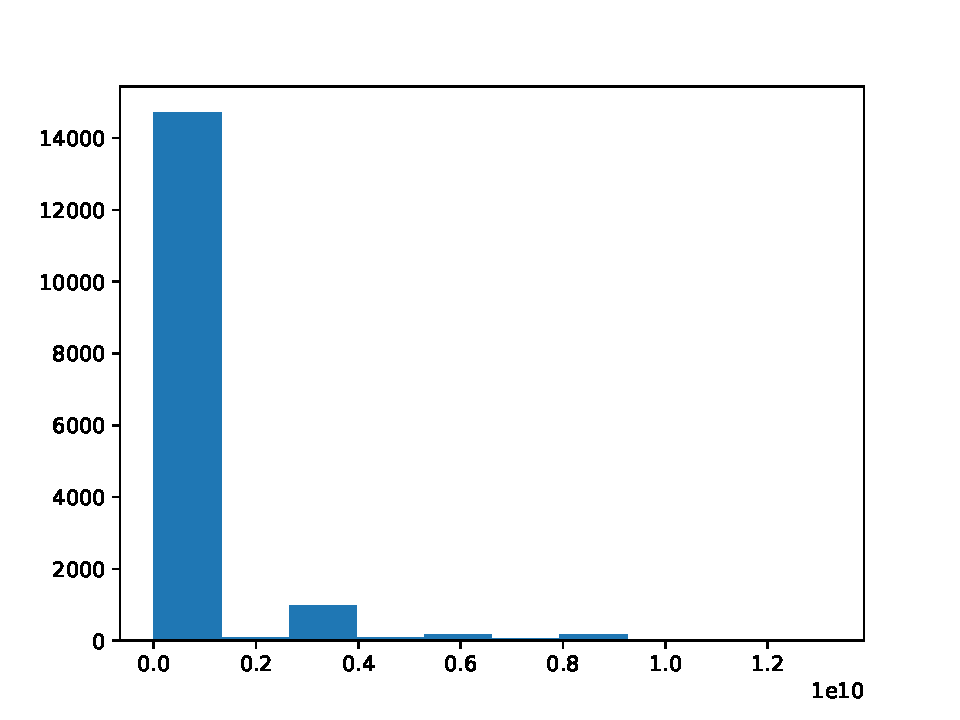
\includegraphics[width=\textwidth]{../../Output/Plots/brand_var.pdf}

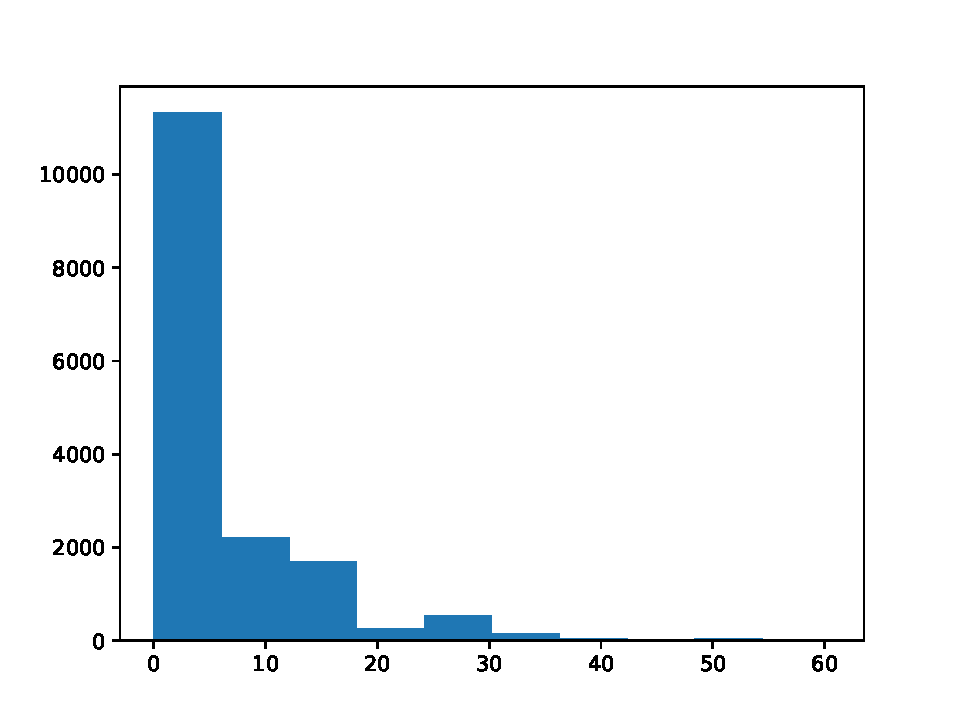
\includegraphics[width=\textwidth]{../../Output/Plots/flavor_var_hist.pdf}

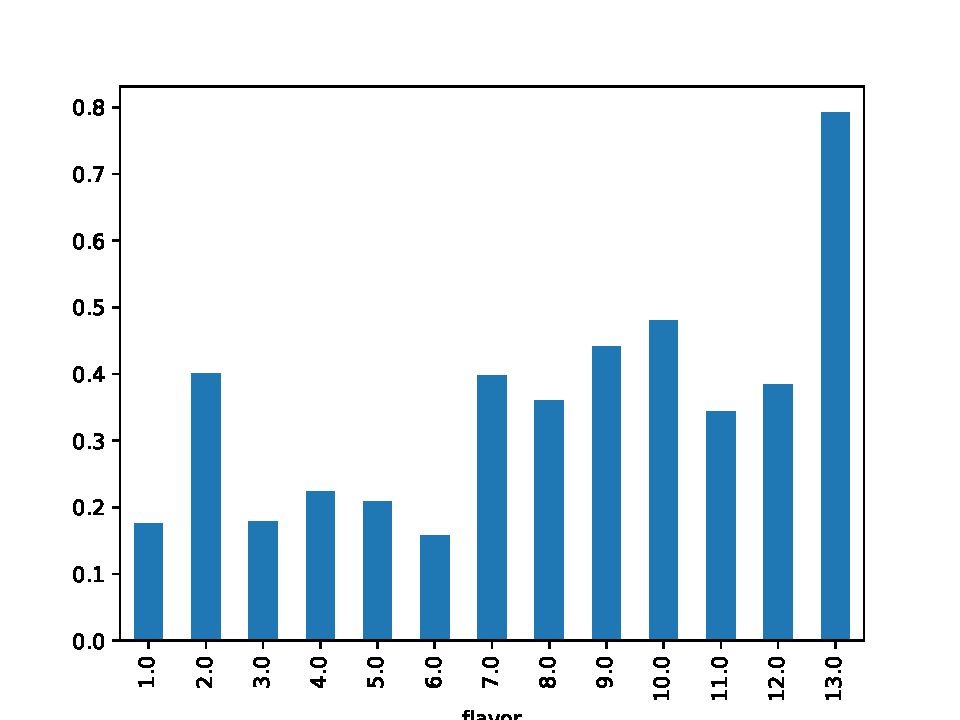
\includegraphics[width=\textwidth]{../../Output/Plots/repeat_flavor_bar.pdf}

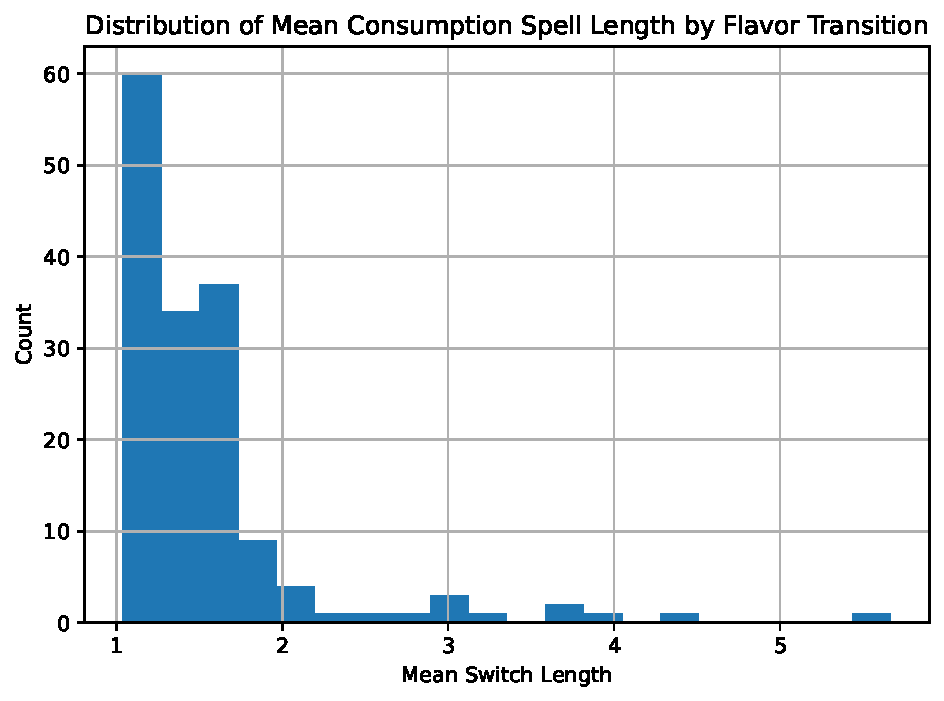
\includegraphics[width=\textwidth]{../../Output/Plots/run_length_hist.pdf}

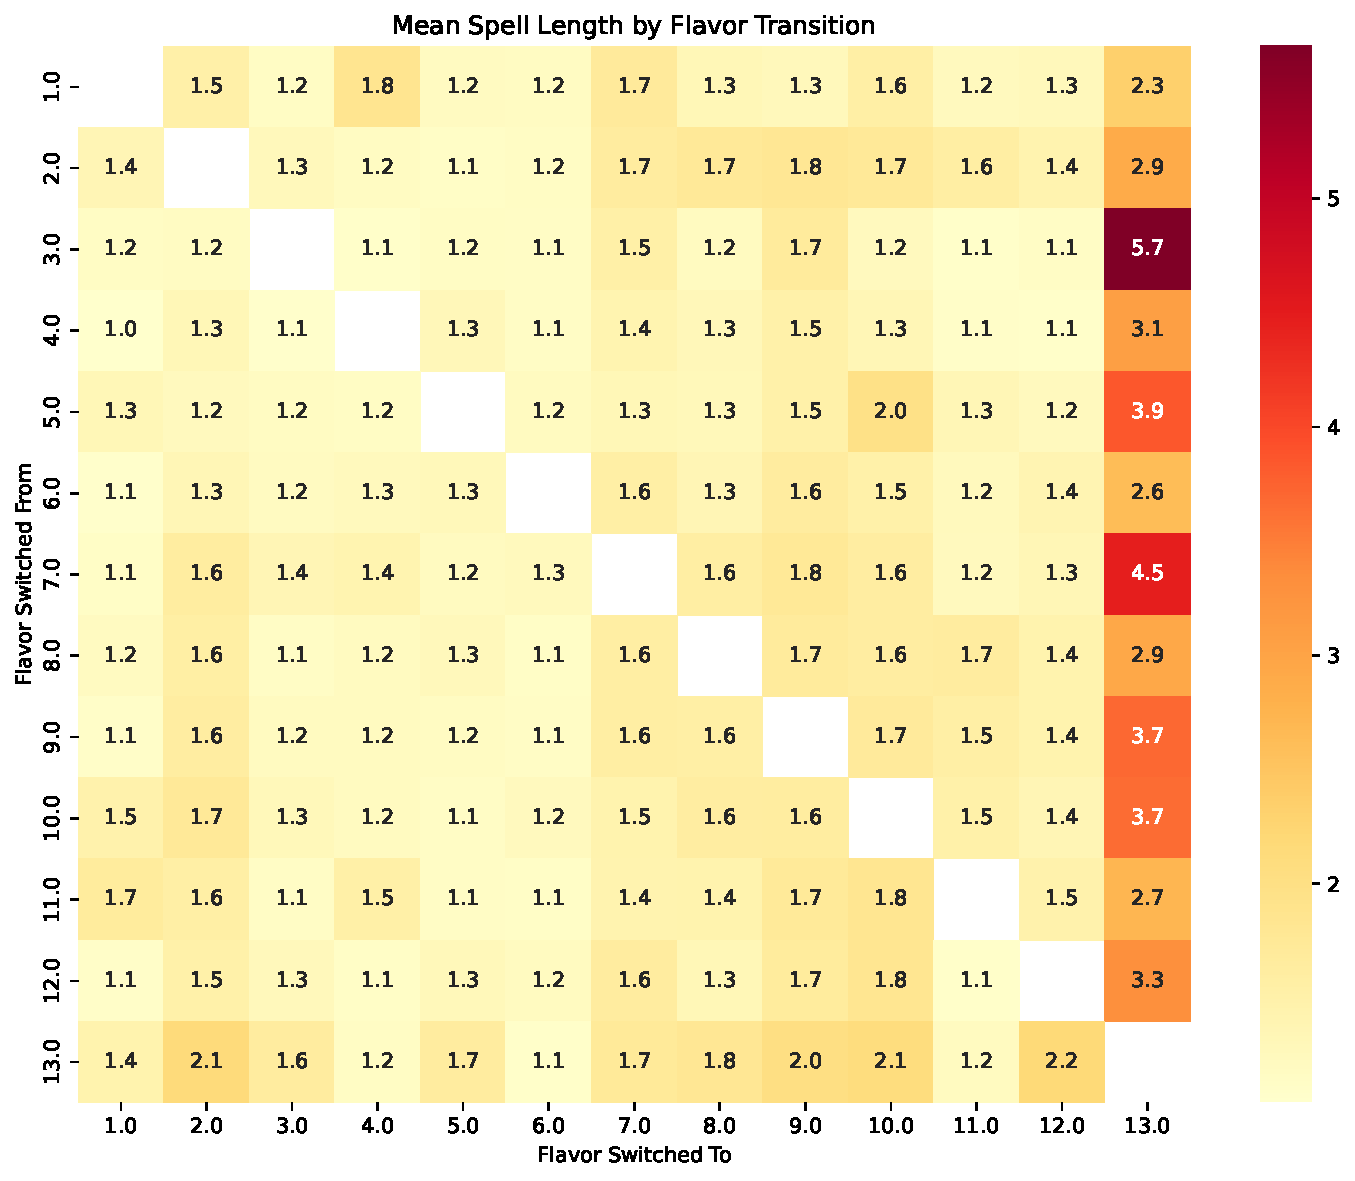
\includegraphics[width=\textwidth]{../../Output/Plots/run_length_heatmap.pdf}

The two final graphs are new. With the first showing the distribution of how
long people stay switched, with most households between one and one and a half
periods. The heatmap shows the transitions. Most households are switching to
plain, and staying on a flavor for 1-2 periods. Strawberry (10) is the most popular
switch, with households staying between 1.5-2 periods. 


\section{Concluding and Next Steps}
Any input would be great. Next, I want to divide by HH demographics to see if
switching differs by things like income or race. I also think that continuing to
formalize the transition matrix of flavors is important as it feels like it will
be a useful statistic when we get to estimation.

\end{document}


